\chapter{Introdução}

 No ano de 2015 a Organização das Nações Unidas (ONU) estimou um índice  de crescimento populacional que relatou a população mundial com 7,3 bilhões de habitantes na metade do ano de 2015, e  demonstrou, ainda, uma prospecção para o ano de 2030 que relata um aumento de 1,2 bilhões no número de habitantes, ou seja a população chegará a
8,5 bilhões \cite {ONU}. 

Aproveitando este contexto de crescimento populacional, tem-se a necessidade do aumento da produção de alimentos, uma vez que, tem-se maior demanda. Com isso, o setor de alimentos é o ramo que mais cresce no Brasil e no mundo. O ramo alimentício possui um acirramento da competição 
devido à grande segmentação da indústria de alimentos. Isso implica que o uso de tecnologias facilita, aprimora e diversifica o mercado. \cite{IBIA}

A proposta do projeto agrega tecnologia e inovação por meio de uma máquina do tipo \textit{Vending Machine} para picolés que pode ser deslocada com facilidade, é alimentada por placas solares, possui \textit{software}, sistema de controle e automação integrados.

\section{Problemática}

Segundo uma entrevista realizada pelos membros da equipe com a empresária Uilma Ribeiro, proprietária da indústria Saborizze®, um freezer comum da Mercofricon 8/A possui 400W de potência e consumo de energia de 3,8kW/24h e faixa de tensão de 220V/60Hz e este consome muito para congelar e manter picolé. Quando se trata do congelamento de placas que mantém o carrinho de picolé referente a figura \ref{fig:carrinho}, este freezer consome ainda mais, uma vez este deve recongelar a placa que descongelou durante o dia na venda, isto aumenta os gastos da indústria distribuidora. Ademais, a empresa deve pagar por custos com funcionários para distribuição e para vendas. 

\begin{figure}[htb]
	\centering
    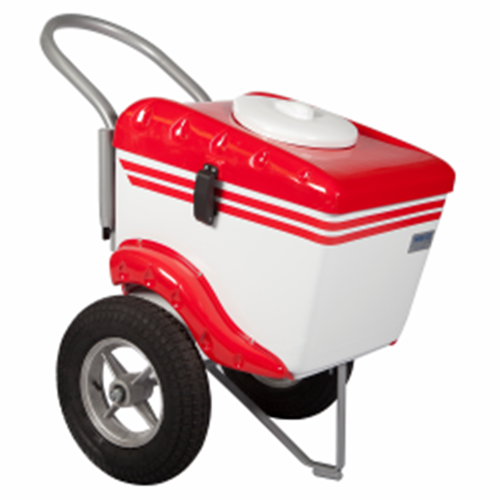
\includegraphics[scale=0.3]{figuras/carrinho}
    \label{fig:carrinho}
    \caption{Carrinho de picolé da indústria Saborizze}
\end{figure}


Visando um diferencial no método de vendas para o mercado competitivo atual no setor alimentício, o projeto $\pi col\acute{e}$ atenderá de forma automática o cliente permitindo acesso prático, metodologia sustentável, diversificação de público e distribuição rápida.

O problema em conjunto com suas causas, estão representados em um diagrama do tipo \textit{FishBone}, também conhecido como diagrama de causa e efeito, o qual é demonstrado na Figura \ref{fig:fishbone}. 

\begin{figure}[htb]
	\centering
    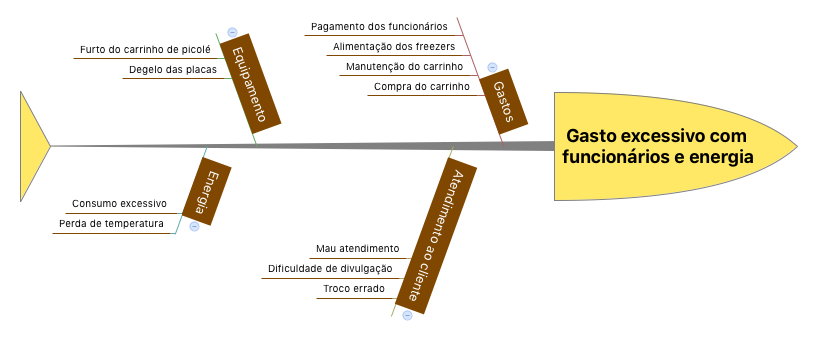
\includegraphics[keepaspectratio=true,scale=0.4]{figuras/fishbone}
    \label{fig:fishbone}
    \caption{Fishbone}
\end{figure}


Para uma descrição sucinta do problema, utilizou-se o seguinte \textit{framework}:

\textbf{O problema:} Gasto excessivo com funcionários e energia.

\textbf{Afeta:} Indústrias de sorvete e sorveteria.

\textbf{Cujo impacto é:} Impacto ambiental devido ao consumo de energia, aumento do preço do produto e diminuição da qualidade do produto final.

\textbf{Uma solução bem sucedida seria:} A criação de uma Vending Machine, a qual automatiza a venda dos picolés sendo possível colocá-la em m diversos pontos de uma cidade.

\section{Estado da Arte}

Existem diversos estilos de venda, como direta, corporativa, casada, consignada e consultiva, considerando o tipo de venda direta, o qual é possível aumentar as vendas, aborda-se um sistema de comercialização de bens de consumo e serviço singular, por meio do contato entre que acontece entre vendedores e compradores sem a necessidade de um estabelecimento físico ou mesmo fixo. \cite {MARQUES} 

Analisando os tipos de venda, e aderindo ao método direto, a utilização de uma máquina do estilo \textit{Vending Machine} se destaca para o projeto $\pi col\acute{e}$. Uma  \textit{Vending Machine} é uma máquina automática que oferece diversos tipos de produtos como cafés, doces, salgados e bebidas sem contato manual para a liberação dos consumíveis, ou seja, são máquinas de autosserviço. Esse tipo de máquina pode ser observada na figura \ref{fig:vending_machine}.
	Esse tipo de\textit{ Vending Machine} é normalmente alimentada pela rede em 220V, com uma interface simples e direta com o usuário, apresenta normalmente um consumo elevado de energia, quando acompanhada de um sistema de refrigeração para venda de produtos gelados.

\begin{figure}[H]
	\centering
    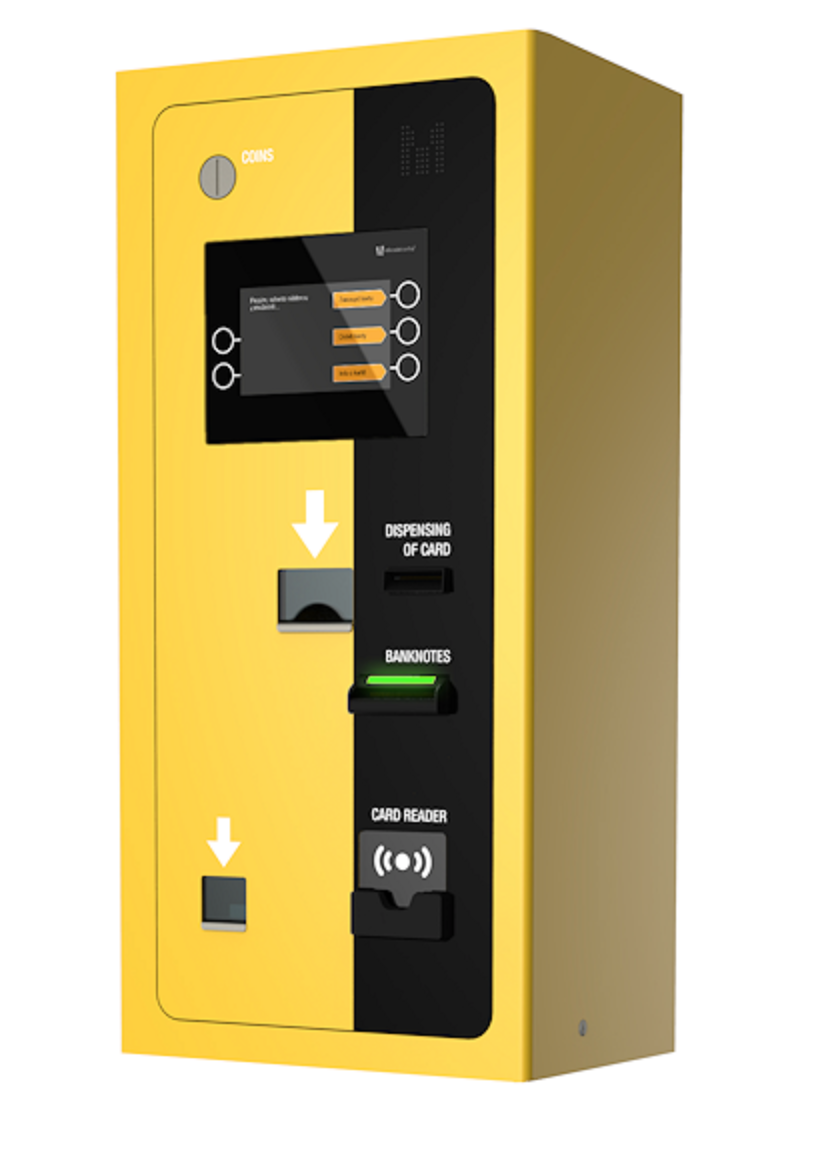
\includegraphics[scale=0.8]{figuras/vending_machine}
    \label{fig:vending_machine}
    \caption{Vending Machine $\pi col\acute{e}$}
\end{figure}

Segundo o manual da ROBO QUENCHER as especificações de potência, dimensões e refrigeração são especificados, sendo assim,para 120v,60 hz, 11amps, 1320watts e para  230v, 50hz, 5amps, 1150watts de potência, com altura de 1830mm, profundidade de 864mm e largura de 1130mm de dimensões e um Compressor de 2 Cavalos, usando um fluido refrigerante R134A, peso de 0,37 kg, e pressões do projeto no lado alto de 200 psi e no lado baixo de 135 psi. A partir dessas informções e dentre outras pesquisadas o $\pi col\acute{e}$ apresenta funcionalidades semelhates de acordo com a especificação do projeto, acrescentando aspectos como vendas por cartão de crédito por meio do  \textit{webapp}, controle de estoque, mecanismo de liberação por mola, relatório de valores aferidos de temperatura e controle, alimentação por painéis fotovoltaicos, autonomia de seis horas, estrutura diferenciada e inovadora.
 \cite{ROBOQUENCHER}



Além disso, utiliza-se uma logo desenvolvida pela equipe de projeto para influenciar na venda do protótipo para indústrias de sorvete e sorveterias. A logo é demonstrada na figura \ref{fig:logopicole}.

\begin{figure}[H]
	\centering
    
\includegraphics[scale=0.2]{figuras/logo_picole}
    \label{fig:logopicole}
    \caption{Logo do projeto $\pi col\acute{e}$}
\end{figure}

As cores escolhidas remetem a sustentabilidade, a alegria e praticidade oferecidas pelo protótipo do projeto. 

\section{Justificativa}

Um sistema que conquiste o cliente, seja prático, atrativo, sustentável, seguro e tecnológico é a solução para o mercado competitivo atual.
A máquina de vendas além de reduzir custos com desperdício de recursos humanos, visa melhorar significativamente as condições de armazenamento do produto provendo, assim, um aumento das vendas e uma redução de custos a longo prazo.
O protótipo deste projeto é uma inovação no mercado, pois ainda não existe um estilo de máquina de vendas que seja em formato de sorvete, de fácil transporte, além de suportar um determinado período sem precisar de carga. 
Dentre as soluções encontradas e estudadas, o protótipo apresenta chances de mercado, segundo pesquisa realizada com a indústria \textit{ Saborizze}®, e também viabilidade financeira e comercial.
Esse tipo de sistema é protótipo $\pi col\acute{e}$.  

\section{Objetivos}

\subsection{Geral}

O objetivo do projeto é construir uma \textit{Vending Machine} que receba o cliente quando estiver perto, dispor de um\textit{Webapp} capaz de realizar vendas por cartão, controlar estoque, mecanismo de liberação de produto e relatório dos valores aferidos de temperatura e controle.  

\subsection{Específicos}

\begin{itemize}
\item Garantir a integração de todas as engenharias;
\item Garantir que todos os integrantes estejam engajados no projeto;
\item Projetar uma estrutura que não danifique o freezer muitos menos permita o tombamento do mesmo;
\item Validar com segurança a venda autônoma de picolés;
\item Obter um sistema de segurança contra furto eficaz;
\item Receber o cliente de forma agradável;
\item Chamar atenção do consumidor;
\item Certificar-se que a temperatura média do freezer seja -5º Celsius com margem de erro de no máximo 5º pra mais;
\item O veículo deverá ser capaz de manter-se resfriado por um período de aproximadamente 10 horas;
\item O sistema de refrigeração deverá ser totalmente vedado;
\item Utilizar um sistema de software para vendas, controle e relatórios.
\end{itemize}


\section{Escopo}
Afim de contemplar a adversidade identificada e os objetivos explanados pelo grupo,foi definido o escopo geral do projeto. A proposta será atestada por meio do desenvolvimento do produto mínimo viável, utilizando o mesmo como objeto de estudo para obter a solução da problemática envolvida neste trabalho. O produto mínimo contempla então, para fins de prototipação, uma máquina de vendas com as seguintes características:

• Capacidade de realizar a venda de picolés de forma autonoma;

• Capacidade de se resfriar para manter os picolés na temperatura adequada;

• Capacidade de se manter \textit{off-grid} durante o período de venda;

• Capacidade de receber pedidos de compra realizados por meio de um web app;

• Capacidade de efetuar diversas medições da temperatura e umidade do ar em intervalos de tempo predefinidos;

• Sistema vinculado capaz de receber os dados em um arquivo e disponibilizar de forma gráfica o relatório de vendas;
